\documentclass[aspectratio=169]{ctexbeamer}

\usetheme{Madrid}
\beamertemplatenavigationsymbolsempty
%\setbeamertemplate{page number in head/foot}[totalframenumber]
%\setbeamertemplate{navigation symbols}{\footnotesize\usebeamertemplate{page number in head/foot}}

\definecolor{tuna}{rgb}{0.098,0.51,0.996}
\definecolor{thu}{rgb}{0.50,0.36,0.71}

\setbeamercolor{section in toc}{fg=black,bg=white}
\setbeamercolor{item}{fg=tuna,bg=white}
\setbeamercolor{alerted text}{fg=tuna!80!gray}
\setbeamercolor*{palette primary}{fg=tuna!60!black,bg=gray!30!white}
\setbeamercolor*{palette secondary}{fg=tuna!70!black,bg=gray!15!white}
\setbeamercolor*{palette tertiary}{bg=tuna!80!black,fg=gray!10!white}
\setbeamercolor*{palette quaternary}{fg=tuna,bg=gray!5!white}

\setbeamercolor*{sidebar}{fg=tuna,bg=gray!15!white}

\setbeamercolor*{palette sidebar primary}{fg=tuna!10!black}
\setbeamercolor*{palette sidebar secondary}{fg=white}
\setbeamercolor*{palette sidebar tertiary}{fg=tuna!50!black}
\setbeamercolor*{palette sidebar quaternary}{fg=gray!10!white}

%\setbeamercolor*{titlelike}{parent=palette primary}
\setbeamercolor{titlelike}{parent=palette primary,fg=tuna}
\setbeamercolor{frametitle}{bg=gray!10!white}
\setbeamercolor{frametitle right}{bg=gray!60!white}

\setbeamercolor*{separation line}{}
\setbeamercolor*{fine separation line}{}

\setbeamertemplate{sections/subsections in toc}[square]
\setbeamertemplate{items}[square]

\AtBeginSection{\frame{\sectionpage}}
\AtBeginSubsection{\frame{\subsectionpage}}

\usepackage{hyperref}
\usepackage{tikz}
\usepackage{graphicx}
\usepackage{caption}
\usepackage{subcaption}
\usepackage{amssymb}
\usepackage{threeparttable}
\usepackage{booktabs}

\usetikzlibrary{decorations.pathreplacing,calligraphy}
\usetikzlibrary{calc}

\setCJKsansfont{Source Han Sans CN}
\setCJKmonofont{Source Han Sans CN}
\setCJKmainfont{Source Han Serif CN}

\newcommand{\T}[1]{\texttt{#1}}

\title{OpenRigil: 开源 RISC-V 密码学硬件密钥}
\author[郑鈜壬]{\textbf{郑鈜壬}\inst{1} \and 叶泽文\inst{2} \and 刘玖阳\inst{3} \and 党凡\inst{1} \and 高鸣宇\inst{1}}
\institute[]{\inst{1}清华大学 \and \inst{2}浙江大学 \and \inst{3}华中科技大学}
\date{2022-08-25}

\begin{document}

\begin{frame}
\maketitle
\end{frame}

\begin{frame}{破题}
  \begin{itemize}
    \item 各位看官,看到这个标题,你可能有两个疑问:
  \end{itemize}
  \begin{enumerate}
    \item 何为「密码学」「硬件密钥」
    \item 这与「开源」「RISC-V」有啥关系
  \end{enumerate}
\end{frame}

\begin{frame}{目录}
  \begin{itemize}
    \item 密码学硬件密钥 % 需求分析 现有工作 % 不可能平地起高楼
    \item 开源与 RISC-V % 为什么开源,为什么选择 RISC-V
    \item 现有开源项目 % 毕竟我们不可能平地起高楼嘛
    \item 我们的工作\begin{itemize}
      \item 实现 RISC-V 标量密码学扩展 % 本科毕设
      \item 蒙哥马利模乘加速器
      \item USB 1.1 外设 % 突出一个能用就行 % 给个图
      \item 完整系统搭建 % all in chisel (how about all in rust)
    \end{itemize}
    \item FPGA 原型与实验 % 评估 Ed25519,RSA 2048 与 RSA4096(可以接受),以及给个图
    \item 缺陷与讨论 % 我们开诚布公,不够安全,没有随机数生成器,时间关系没写完固件(固件移植),开源这个好处:随着时间增加,总会有的;更多的板子支持
  \end{itemize}
\end{frame}

\section{密码学硬件密钥}
% 说到密码学硬件密钥,大家可能很陌生,这是什么东西
% 简单场景:登录(验证),简单密码,弱密码,密码泄漏
% case study:手机验证码(公钥实名制,之前有工作,当然不在我们讨论范围内了)
% 并不算特别安全的信道
% 另一个简单场景:签名,手写签名,电子签名
% 让我们介绍密码学工具:RSA ECC(详细展开在蒙哥马利)
% 密钥的存放:SSH 私钥(普通文件!)是否有更
% Introduce 硬件安全密钥(其他的例如手机 TOTP)
% 典型产品

\begin{frame}{第一印象}
  \begin{columns}
    \begin{column}{0.5\textwidth}
      \begin{itemize}
        \item 大家可能对这种设备比较陌生
        %\item Yubikey
        \item 第一印象是 U 盘
        \item 但它并不能存一般的文件
        \item 那为什么会需要这种设备
      \end{itemize}
    \end{column}
    \begin{column}{0.5\textwidth}
      \begin{figure}
        \centering
        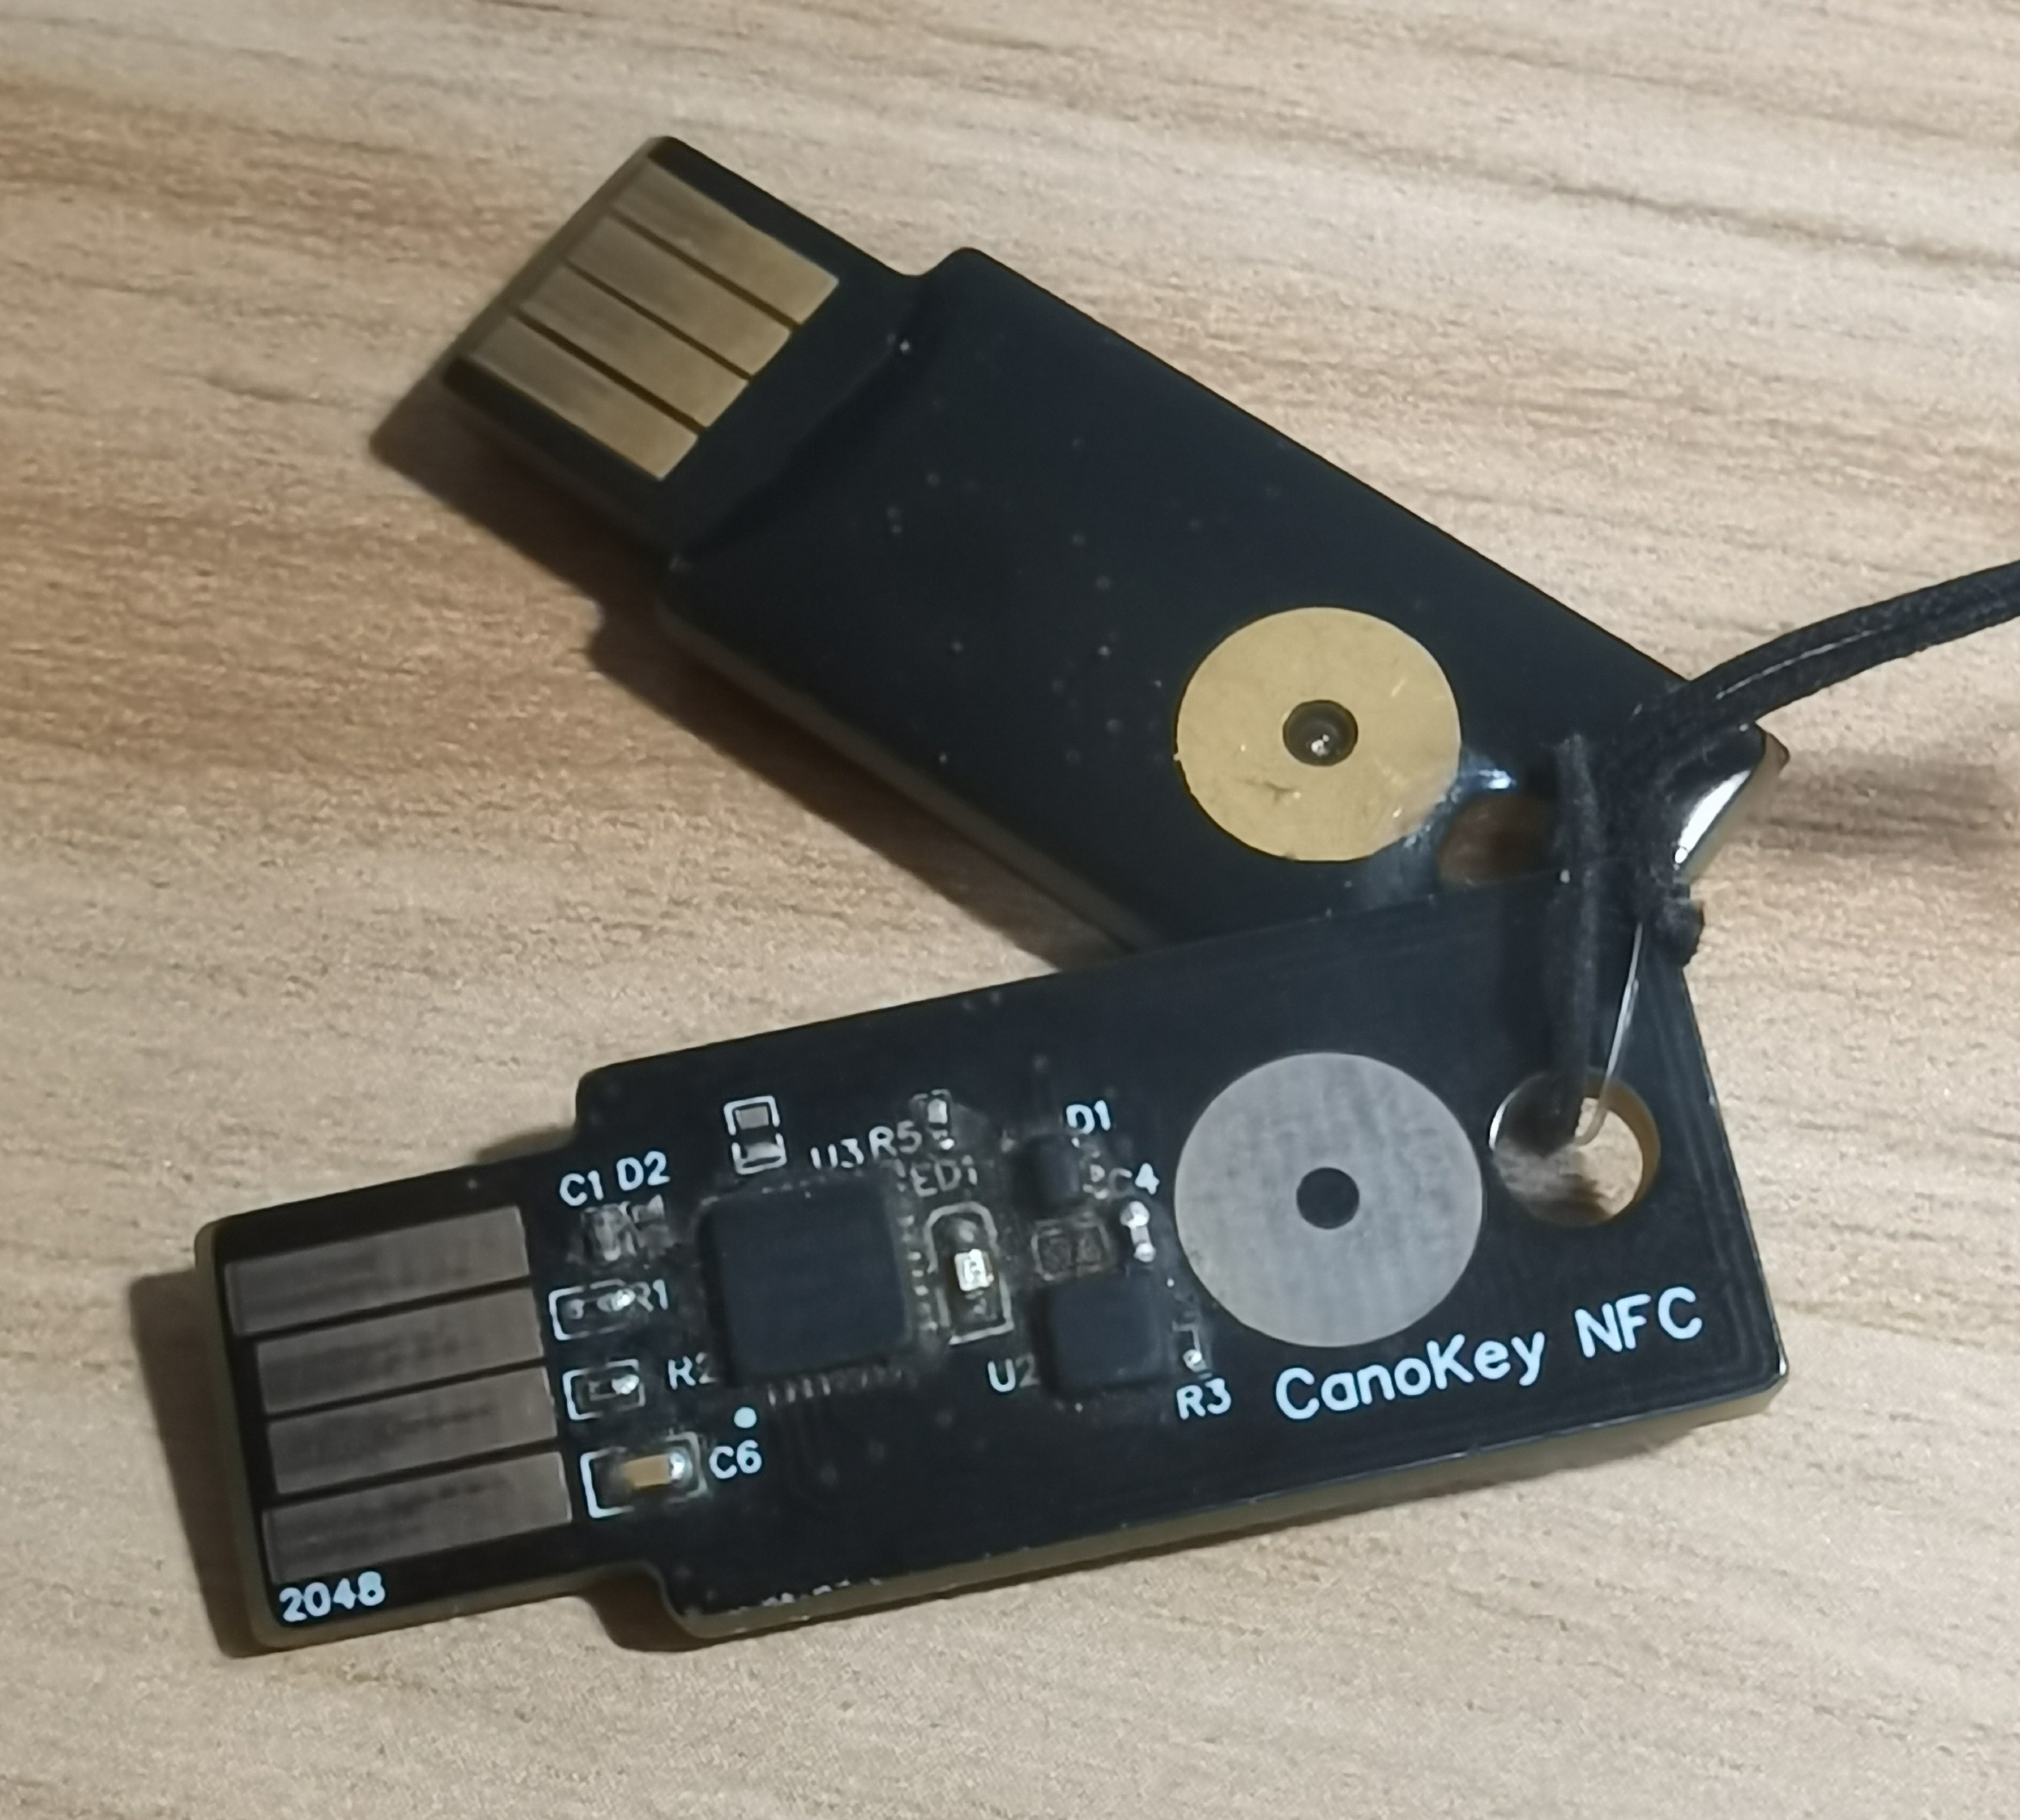
\includegraphics[width=0.7\textwidth]{img/key.jpg}
        \caption{密码学硬件密钥样例}
      \end{figure}
    \end{column}
  \end{columns}
\end{frame}

\begin{frame}{从简单场景出发:密码}
  \begin{itemize}
    \item<1-> 我们来说说帐号密码系统
    \item<1-> 密码是个麻烦的东西
    \item<2-> 想必大家对怎么设置自己各类帐号的密码都各有心得\begin{itemize}
      \item<3-> 弱密码:容易爆破
      \item<3-> 强密码:容易忘记
      \item<3-> 忘记密码:找回密码很麻烦
      \item<4-> 各帐号同一个密码:容易泄漏
      \item<5-> 将密码记在小本本上:不是良好习惯
      \item<5-> 密码管理器:各个设备之间的同步,管理器、服务商是否可信
    \end{itemize}
  \end{itemize}
\end{frame}

\begin{frame}{解决密码的麻烦:多因子验证} % portability
  \begin{columns}
    \begin{column}{0.5\textwidth}
      \begin{itemize}
        \item<1-> 多因子验证(MFA):密码+其他手段(因子)
        % 这并不是一个新鲜的概念
        \item<2-> 多因子验证已经被实践了很久\begin{itemize}
          \item 短信验证码
          \item 扫码登录(其他帐号验证)
          \item 生物因素(人脸识别、指纹)
          \item 软件验证码(Microsoft Authenticator)
        \end{itemize}
        \item<3-> 还有没有别的因子呢?公钥密码学
      \end{itemize}
    \end{column}
    \begin{column}{0.5\textwidth}
      \begin{figure}
        \centering
        
\includegraphics[width=0.6\textwidth]{img/totp.png}
        \caption{验证码样例}
      \end{figure}
    \end{column}
  \end{columns}
\end{frame}

\begin{frame}{另一个场景:电子签名}
  \begin{columns}
    \begin{column}{0.4\textwidth}
      \begin{itemize}
        \item 签名自古以来的难题:伪造
        \begin{itemize}
          \item 手写签字
          \item 盖章
        \end{itemize}
        \item 公钥密码学签名\begin{itemize}
          % 攻壳机动队
          \item 密码学认为难以伪造
        \end{itemize}
      \end{itemize}
    \end{column}
    \begin{column}{0.6\textwidth}
      \begin{figure}
        \centering
        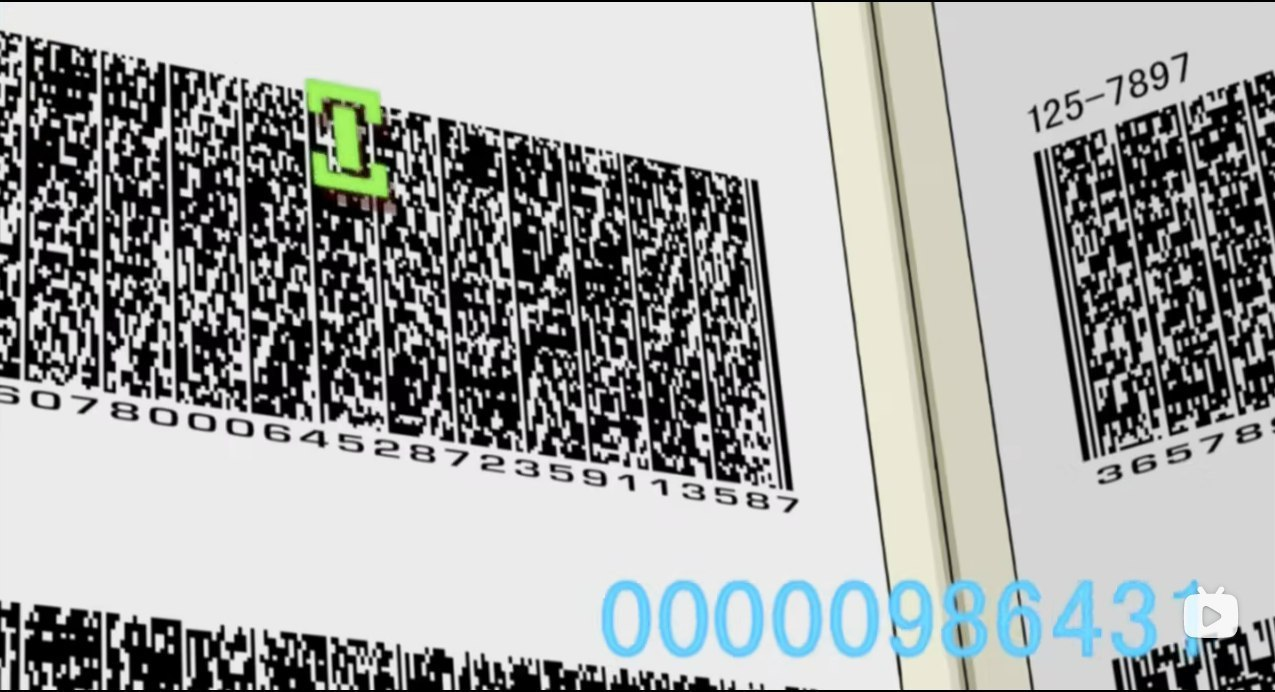
\includegraphics[width=0.8\textwidth]{img/base64.jpg}\footnote{图自《攻壳机动队》,图文无关}
      \end{figure}
    \end{column}
  \end{columns}
\end{frame}

\begin{frame}{公钥密码学}
  \begin{center}
    \begin{tikzpicture}
      \node at (-2,0) {服务器};
      \node at (2,0) {用户};
      \draw[thick,->] (-1.5,-1) -- node[above] {消息} (1.5,-1);
      \node[draw,thick] at (2.5,-1.5) {私钥签名};
      \draw[thick,->] (1.5,-2) -- node[below] {签名} (-1.5,-2);
      \node[draw,thick] at (-2.5,-1) {生成};
      \node[draw,thick] at (-2.5,-2) {公钥验证};
    \end{tikzpicture}
  \end{center}
  \begin{itemize}
    \item<1-> 注册:用户生成私钥与公钥,并讲公钥提交给服务器
    \item<2-> 登录:服务器生成消息,让用户签名,如果该签名能通过公钥检验,则可以登录
    \item<3-> 密码学认为:难以通过公钥计算私钥,难以伪造签名
    \item<3-> 常见公钥密码学实现:RSA 与 ECC(椭圆曲线密码学) % PQC
  \end{itemize}
\end{frame}

\begin{frame}{公钥密码学很好,但还不够}
  % 图:应用与私钥匙放在一块
  \begin{columns}
    \begin{column}{0.5\textwidth}
      \begin{itemize}
        \item 用户私钥怎么存放,怎么管理
        \item<2-> 人脑记忆、人脑计算\begin{itemize}
          \item 人脑算 RSA4096
          \item 请您上最强大脑!
        \end{itemize}
        \item<3-> 私钥存在电脑上,应用旁边\begin{itemize}
          \item 那应用会不会偷偷读取你的私钥
          \item 闭源软件最终会演变成恶意软件
          \item 假如软件偷偷全盘扫描……
        \end{itemize}
        \item<4-> 如何解决
      \end{itemize}
    \end{column}
    \begin{column}{0.5\textwidth}
      \begin{center}
        \only<2>{\begin{figure}
          \centering
          
\includegraphics[width=0.5\textwidth]{img/nano.png}
          \caption{最强大脑}
        \end{figure}}
        \only<3,4>{\begin{tikzpicture}
          \draw[thick] (0,0) -- (4,0) -- (4,3) -- (0,3) -- (0,0);
          \node at (2,2) {操作系统};
          \node[draw,thick] (App) at (1,1) {应用};
          \node[draw,thick] (Pri) at (3,1) {私钥};
          \draw[red,thick,->] (Pri) -- node[above] {扫描} node[below] {$\checkmark$} (App);
        \end{tikzpicture}}
      \end{center}
    \end{column}
  \end{columns}
\end{frame}

\begin{frame}{硬件密钥}
  % 图:接口与不允许导出
  \begin{columns}
    \begin{column}{0.5\textwidth}
      \begin{itemize}
        \item 将私钥放在「硬件密钥」上
        \item 接口保证不导出私钥,只允许签名
        \item 签名的时候需要用户交互
        \item 保护了私钥
        %\item 并没有说绝对安全,只是相对更难破解
        %\item 只要验证接口是安全的,以及验证固件和硬件是安全的
        %\item 比较可惜的是,国内支持硬件密钥的帐号系统较少(讨论范围之外)
        %\item 可惜尚未被国内系统大量使用 % 公钥实名制能做吗? 不知道的因素,这是今天讨论范围之外的问题
      \end{itemize}
    \end{column}
    \begin{column}{0.5\textwidth}
      \begin{center}
        \begin{tikzpicture}
          \draw[thick] (0,0) -- (3,0) -- (3,2) -- (0,2) -- (0,0);
          \node at (1.5,1.33) {操作系统};
          \node[draw,thick] (App) at (1.5,0.67) {应用};
          \draw[thick] (0,-3) -- (3,-3) -- (3,-1) -- (0,-1) -- (0,-3);
          \node at (1.5,-2.33) {硬件密钥};
          \node[draw,thick] (Pri) at (1.5,-1.67) {私钥};
          \draw[color=black!40!green,->,thick] (Pri) to [bend left] node[left]{签名 $\checkmark$} (App);
          \draw[color=red,->,thick] (Pri) to [bend right] node[right]{导出 $\times$} (App);
        \end{tikzpicture}
      \end{center}
    \end{column}
  \end{columns}
\end{frame}

\begin{frame}{「密码学」硬件密钥}
  \begin{columns}
    \begin{column}{0.6\textwidth}
      \begin{itemize}
        \item<1-> 密码学运算需要的计算量大
        \item<1-> 例如不使用硬件加速在嵌入式芯片 或 FPGA 上用 RSA4096 签名,需要 20 秒
        \item<2-> 想象你正在赶 DDL,23:59 交作业
        \item<2-> 现在是 23:58,你正在登录系统,事态非常紧急
        \item<2-> 结果登录的时候在等签名……
        \item<3-> 所以需要「密码学」硬件密钥
        \item<3-> 即搭载密码学加速器的硬件密钥
      \end{itemize}
    \end{column}
    \begin{column}{0.4\textwidth}
      \begin{figure}
        \centering
        
\includegraphics[width=0.8\textwidth]{img/99.png}\footnote{Capoo}
      \end{figure}
    \end{column}
  \end{columns}
\end{frame}

\begin{frame}{密码学硬件密钥架构}
  \begin{center}
    \begin{tikzpicture}[x=1.5cm]
      \node (Hardware) at (-4, 2) {运算};
      \node[draw,thick,fill=white,minimum width=5cm] (Core) at (-1.8, 2) {核心};
      \node[draw,thick,fill=white,minimum width=5cm] (Accelerator) at (1.8, 2) {加速器};
      \node (Crypto) at (-4, 1) {密码};
      \node[draw,thick,fill=white] (RNG) at (-3, 1) {RNG};
      \node[draw,thick,fill=white] (AES) at (-2, 1) {AES};
      \node[draw,thick,fill=white] (DES) at (-1, 1) {DES};
      \node[draw,thick,fill=white] (RSA) at (0, 1) {RSA};
      \node[draw,thick,fill=white] (ECC) at (1, 1) {ECC};
      \node[draw,thick,fill=white] (SHA) at (2, 1) {SHA};
      \node[draw,thick,fill=white] (HMAC) at (3, 1) {HMAC};
      \node (App) at (-4, 0) {应用};
      \node[draw,thick,fill=white] (OpenPGP) at (-3, 0) {OpenPGP};
      \node[draw,thick,fill=white] (PIV) at (-1.9, 0) {PIV};
      \node[draw,thick,fill=white] (OATH) at (-1, 0) {OATH};
      \node[draw,thick,fill=white] (CTAP) at (0, 0) {CTAP};
      \node[draw,thick,fill=white] (ADMIN) at (1, 0) {Admin};
      \node[draw,thick,fill=white] (NDEF) at (2, 0) {NDEF};
      \node[draw,thick,fill=white] (Meta) at (3, 0) {Meta};
      \node (Transport) at (-4, -1) {指令};
      \node[draw,thick,fill=white,minimum width=5cm] (APDU) at (-1.8, -1) {APDU};
      \node[draw,thick,fill=white,minimum width=5cm] (FS) at (1.8, -1) {文件系统调用};
      \node (Driver) at (-4, -2) {驱动};
      \node[draw,thick,fill=white,minimum width=5cm] (WebUSB) at (-1.8, -2) {USB WebUSB/CCID/HID};
      \node[draw,thick,fill=white,minimum width=5cm] (Flash) at (1.8, -2) {SPI Flash};
      \node (Transport) at (-4, -3) {传输};
      \node[draw,thick,fill=white,minimum width=5cm] (USB) at (-1.8, -3) {USB};
      \node[draw,thick,fill=white,minimum width=5cm] (SPI) at (1.8, -3) {SPI};
      %
      \draw [ultra thick,decorate,
          decoration={calligraphic brace,raise=5pt,amplitude=5pt,mirror}] (3.6,-2) --  (3.6,0);
      %
      \node (Protocol) at (4.7, -1) {协议栈(软件)};
      \node (Crypto) at (4.7, 1) {密码库(软件)};
      \node (Periphery) at (4.7, -3) {外设(硬件)};
      \node (Hardware) at (4.7, 2) {处理器(硬件)};
      %
      \node<1,3> at (-1.8,-4) {用户请求}; \node<1>[fill=white,color=white] at (-1.8,-4) {用户请求};
      \node<2,4>[color=red] at (-1.8,-4) {用户请求}; 
      \node<5> at (1.8,-4) {私钥}; \node<1,2>[fill=white,color=white] at (1.8,-4) {私钥};
      \node<3,4>[color=red] at (1.8,-4) {私钥}; 
      %
      \draw<2,4>[red,thick,->] (USB) -- (WebUSB); \draw<3>[thick,->] (USB) -- (WebUSB);
      \draw<2,4>[red,thick,->] (WebUSB) -- (APDU); \draw<3>[thick,->] (WebUSB) -- (APDU);
      \draw<2,4>[red,thick,->] (APDU) -- (-1.8, -0.4); \draw<3>[thick,->] (APDU) -- (-1.8, -0.4);
      %
      \draw<3>[red,thick,->] (1.8, -0.4) -- (FS);
      \draw<4>[red,thick,->] (FS) -- (1.8, -0.4); \draw<5->[thick,->] (FS) -- (1.8, -0.4);
      \draw<3>[red,thick,->] (FS) -- (Flash);
      \draw<4>[red,thick,->] (Flash) -- (FS); \draw<5->[thick,->] (Flash) -- (FS);
      \draw<3>[red,thick,->] (Flash) -- (SPI);
      \draw<4>[red,thick,->] (SPI) -- (Flash); \draw<5->[thick,->] (SPI) -- (Flash);
      %
      \draw<4>[red,thick,->] (0, 0.3) -- (0, 0.7);
      \draw<4>[red,thick,->] (0, 1.3) -- (0, 1.7);
      %
      \draw<5>[red,thick,->] (0, 0.7) -- (0, 0.3);
      \draw<5>[red,thick,->] (0, 1.7) -- (0, 1.3);
      \draw<5>[red,thick,->] (-1.8, -0.4) -- (APDU);
      \draw<5>[red,thick,->] (APDU) -- (WebUSB);
      \draw<5>[red,thick,->] (WebUSB) -- (USB);
      \node<5>[color=red] at (-1.8,-4) {签名};
    \end{tikzpicture}
  \end{center}
\end{frame}

%\begin{frame}{密钥管理} % portability
%  \begin{itemize}
%    \item<1-> 我们有很多密钥\begin{itemize}
%      \item 密码(网站密码,开机密码等)
%      \item SSH 密钥(例如 \T{\~{}/.ssh/id\_rsa})
%      \item X.509 证书(签名、解密、认证)
%      \item OpenPGP 密钥(签名、解密、认证)
%    \end{itemize}
%    \item<2-> 难以管理\begin{itemize}
%      \item<3-> 难以记忆:密码,4096 位的 SSH 密钥
%      \item<4-> 难以隔离:你运行的所有程序(包括你不信任的程序)都能够读取到,操作系统不阻拦\begin{itemize}
%        \item 你运行的联网软件能够读取并上传你的 SSH 私钥!
%      \end{itemize}
%      \item<5-> 难以迁移\begin{itemize}
%        \item 一台机器的密钥如何安全拷贝到另一台机器上(聊天软件分发?)
%        \item 一台电脑遗失了需要吊销所有电脑的密钥
%      \end{itemize}
%    \end{itemize}
%    \item<6-> CanoKey 提供隔离(不可导出密钥)且便携的硬件密钥
%  \end{itemize}
%\end{frame}

% 密码学硬件密钥特性:性能有限,NFC 能量有限
% 我们不开心,我们要做了!我们先来做一下需求分析
% 目标:跑通就行,性能和功能都不怕,反正不卖,也是开源的(社区开心了会自己贡献)
% 需求分析:公钥密码学(重头戏):不可能让用户等(21s,stm32 纯软件版 15s)
% 核:基本是 ARM 核,也不开源
% 加速器:不开源,是吃饭的东西
% SoC:外设和各类驱动,这往往不在开源的考虑范围内,即使核开源了外设也不一定开源

\section{开源与 RISC-V}
% 我来这,只追求三件事:开源,开源,还是开源
% 与讲私钥放在电脑一样危险一样,将私钥放在密码学硬件密钥上也不一定安全
% 开源是可信的底线,没有开源不谈可信
% 不光是固件开源,硬件也需要开源,不仅 ISA 开源,核开源,外设与 SoC 也要开源
% 还要做开源加速器

\begin{frame}{现有产品:不够开源}
  \begin{itemize}
    \item 我来峰会,只办三件事:开源、开源、还是开源
    \item 之前说到,密码学硬件密钥保护了私钥
    \item 这是建立在密码学硬件密钥「可信」的基础上的
    \item 我认为「开源」是「可信」的最低要求\begin{itemize}
      \item 可供用户与开发者审计,找出潜在的问题
      \item 能较大程度上避免植入恶意后门
    \end{itemize}
    \item<2> 现有产品最多做到固件开源,硬件开源难以做到\begin{itemize}
      \item YubiKey:核,加速器,固件均不开源
      \item STM32 阵营(NitroKey/SoloKey):固件开源但 ARM 核不开源
      \item nRF52 阵营(OpenSK):ARM 核、密码学加速器不开源
      %\item OpenTitan: emm,还在做硬件,软件还没做完(放到最后讨论)
    \end{itemize}
    %\item 不过,要做到全部开源并不容易:软件开源,密码学开源,硬件开源,SoC 开源,加速器开源
  \end{itemize}
\end{frame}

\begin{frame}{RISC-V 的天然优势}
  \begin{itemize}
    \item RISC-V 峰会,当然还是要吹一波 RISC-V 的
    \item 不过说实话,这个项目能成,主要还是 RISC-V 有基础设施
    \item 我们能够自由使用 RISC-V ISA 和相应工具链
    \item 我们能够自由选择开源 RISC-V 核,例如 rocket-chip, cva6
    \item 相关的开源外设也较为方便使用
  \end{itemize}
\end{frame}

\begin{frame}{我们的目标}
  \begin{columns}
    \begin{column}{0.5\textwidth}
      \begin{itemize}
        \item 我们要做开源硬件密钥
        \item 我们追求:全部开源\begin{itemize}
          \item RISC-V 核心开源
          \item 加速器开源
          \item 外设开源
          \item 密码学库开源
          \item 协议栈开源
        \end{itemize}
      \end{itemize}
    \end{column}
    \begin{column}{0.5\textwidth}
      \begin{center}
        \begin{tikzpicture}
          \draw[thick] (-0.1, 0.1) -- (-0.1, 3.0) -- (-3.0, 3.0) -- (-3.0, 0.1) -- (-0.1, 0.1);
          \draw[thick] (0.1, 0.1) -- (0.1, 3.0) -- (3.0, 3.0) -- (3.0, 0.1) -- (0.1, 0.1);
          \draw[thick] (-0.1, -0.1) -- (-0.1, -3.0) -- (-3.0, -3.0) -- (-3.0, -0.1) -- (-0.1, -0.1);
          \draw[thick] (0.1, -0.1) -- (0.1, -3.0) -- (3.0, -3.0) -- (3.0, -0.1) -- (0.1, -0.1);
          \node (core) at (-1.5, 2.5) {核/加速器};
          \node (pheri) at (1.5, 2.5) {外设};
          \node (Crypto) at (-1.5, -0.5) {密码学库};
          \node (Proto) at (1.5, -0.5) {协议栈};
          %
          \node[align=center] (zk) at (-1.5, 1) {开源};
          \node[align=center] (peri) at (1.5, 1) {开源};
          \node[align=center] (crypto) at (-1.5, -2) {开源};
          \node[align=center] (proto) at (1.5, -2) {开源};
          %\node[align=center] (zk) at (-1.5, 1) {RV32IMACZk \\ MMM 加速器};
          %\node[align=center] (peri) at (1.5, 1) {USB \\ SPI \\ UART};
          %\node[align=center] (crypto) at (-1.5, -2) {RSA ECC \\ AES SHA};
          %\node[align=center] (proto) at (1.5, -2) {FIDO2 OATH \\ OpenPGP PIV};
        \end{tikzpicture}
      \end{center}
    \end{column}
  \end{columns}
\end{frame}

\begin{frame}{我们的限制}
  \begin{itemize}
    \item 时间和人力有限:几个人业余做\begin{itemize}
      \item 以较小的工作,搭建一个跑通的系统,展现这是能做的
    \end{itemize}
    \item 不求尽善尽美\begin{itemize}
      \item 功能不一定最全,性能不一定最优
      \item (比不过比不过,毕竟别人是靠这个吃饭的)
    \end{itemize}
    \item 在峰会上介绍给社区,社区可复现\begin{itemize}
      \item 开源的好处:想加功能,想优化,都可以动手做
    \end{itemize}
  \end{itemize}
\end{frame}

\section{现有开源项目}
% 不可能平地起高楼
% 有人可能会说:这个事情很简单,不是随便抓个核就能做? 
% 的确,开源世界的工作就是搭积木
% 需要什么:协议栈,密码学库,硬件驱动,核,外设
% 缺了一些部件,或者不够用
% 我们想象一个最基础的系统:协议栈:canokey-core,密码学:mbedtls
% 系统:rocket chip,外设:rocket-chip blocks
% 没有密码学加速,以及没有 USB
% 维护者也是我们

\begin{frame}{不可能平地起高楼}
  \begin{columns}
    \begin{column}{0.5\textwidth}
      \begin{itemize}
        \item 自己写核,自己写总线,自己写外设,自己写软件,自己写密码学库,自己写协议栈,自己调试...
        \item 工期来不及\begin{itemize}
          \item 不做个三五年怎么可能做完
          \item 三年综合、五年模拟
        \end{itemize}
        \item 时效性不行
        \item 一定要复用现有开源软件,快速出原型
      \end{itemize}
    \end{column}
    \begin{column}{0.5\textwidth}
      \begin{center}
        \begin{tikzpicture}
          \draw[thick] (-0.1, 0.1) -- (-0.1, 3.0) -- (-3.0, 3.0) -- (-3.0, 0.1) -- (-0.1, 0.1);
          \draw[thick] (0.1, 0.1) -- (0.1, 3.0) -- (3.0, 3.0) -- (3.0, 0.1) -- (0.1, 0.1);
          \draw[thick] (-0.1, -0.1) -- (-0.1, -3.0) -- (-3.0, -3.0) -- (-3.0, -0.1) -- (-0.1, -0.1);
          \draw[thick] (0.1, -0.1) -- (0.1, -3.0) -- (3.0, -3.0) -- (3.0, -0.1) -- (0.1, -0.1);
          \node (core) at (-1.5, 2.5) {核/加速器};
          \node (pheri) at (1.5, 2.5) {外设};
          \node (Crypto) at (-1.5, -0.5) {密码学库};
          \node (Proto) at (1.5, -0.5) {协议栈};
          %
          \node[align=center] (zk) at (-1.5, 1) {自己做?};
          \node[align=center] (peri) at (1.5, 1) {自己做?};
          \node[align=center] (crypto) at (-1.5, -2) {自己做?};
          \node[align=center] (proto) at (1.5, -2) {自己做?};
        \end{tikzpicture}
      \end{center}
    \end{column}
  \end{columns}
\end{frame}

\begin{frame}{还差那么……一点点}
  \begin{columns}
    \begin{column}{0.5\textwidth}
      \begin{itemize}
        \item 一些观众:这不是随便抓一些项目来就能跑通
        \item 我们来假想一下要选哪些\begin{itemize}
          \item<1-> 核:rocket chip, cva6, ibex...
          \item<2-> 加速器:并不完全符合需求
          \item<3-> 外设:随便找一些开源外设
          \item<4-> 密码学库:MbedTLS/OpenSSL,无 RSA/ECC 硬件加速
          \item<5-> 协议栈:Yubikey-neo,NitroKey, Gnuk...
        \end{itemize}
        \item<6> 还差那么……一点点
      \end{itemize}
    \end{column}
    \begin{column}{0.5\textwidth}
      \begin{center}
        \begin{tikzpicture}
          \draw[thick] (-0.1, 0.1) -- (-0.1, 3.0) -- (-3.0, 3.0) -- (-3.0, 0.1) -- (-0.1, 0.1);
          \draw[thick] (0.1, 0.1) -- (0.1, 3.0) -- (3.0, 3.0) -- (3.0, 0.1) -- (0.1, 0.1);
          \draw[thick] (-0.1, -0.1) -- (-0.1, -3.0) -- (-3.0, -3.0) -- (-3.0, -0.1) -- (-0.1, -0.1);
          \draw[thick] (0.1, -0.1) -- (0.1, -3.0) -- (3.0, -3.0) -- (3.0, -0.1) -- (0.1, -0.1);
          \node (core) at (-1.5, 2.5) {核/加速器};
          \node (pheri) at (1.5, 2.5) {外设};
          \node (Crypto) at (-1.5, -0.5) {密码学库};
          \node (Proto) at (1.5, -0.5) {协议栈};
          %
          \node[align=center] (zk) at (-1.5, 1) {{\color{black!40!green}RV32IMAC}{\color{orange}Zk} \\ {\color{orange}MMM 加速器}};
          \node[align=center] (peri) at (1.5, 1) {{\color{orange}USB} \\ {\color{black!40!green}SPI} \\ {\color{black!40!green}UART}};
          \node[align=center] (crypto) at (-1.5, -2) {\color{orange}RSA ECC \\ \color{black!40!green}AES SHA};
          \node[align=center] (proto) at (1.5, -2) {\color{black!40!green}FIDO2 OATH \\ \color{black!40!green}OpenPGP PIV};
        \end{tikzpicture}
      \end{center}
    \end{column}
  \end{columns}
\end{frame}

\begin{frame}{我们的选择}
  \begin{columns}
    \begin{column}{0.5\textwidth}
      \begin{itemize}
        \item<1-> 基础选择\begin{itemize}
          \item rocket-chip(刘玖阳是现有维护者)
          \item rocket-chip-blocks(旧称 sifive-blocks) 的 SPI/UART 外设
          \item canokey-core(党凡是主要作者)
        \end{itemize}
        \item<2> 我们的工作\begin{itemize}
          \item 为 rocket-chip 增加标量密码学扩展 Zk 的支持
          \item 公钥密码学蒙哥马利模乘加速器
          \item 与 Zk、模乘加速器相对应的密码学库
          \item USB 1.1 外设
          \item 完整系统搭建
        \end{itemize}
      \end{itemize}
    \end{column}
    \begin{column}{0.5\textwidth}
      \begin{center}
        \begin{tikzpicture}
          \draw[thick] (-0.1, 0.1) -- (-0.1, 3.0) -- (-3.0, 3.0) -- (-3.0, 0.1) -- (-0.1, 0.1);
          \draw[thick] (0.1, 0.1) -- (0.1, 3.0) -- (3.0, 3.0) -- (3.0, 0.1) -- (0.1, 0.1);
          \draw[thick] (-0.1, -0.1) -- (-0.1, -3.0) -- (-3.0, -3.0) -- (-3.0, -0.1) -- (-0.1, -0.1);
          \draw[thick] (0.1, -0.1) -- (0.1, -3.0) -- (3.0, -3.0) -- (3.0, -0.1) -- (0.1, -0.1);
          \node (core) at (-1.5, 2.5) {核/加速器};
          \node (pheri) at (1.5, 2.5) {外设};
          \node (Crypto) at (-1.5, -0.5) {密码学库};
          \node (Proto) at (1.5, -0.5) {协议栈};
          %
          \node[align=center] (rocket) at (-1.5, 2) {\color{brown}rocket-chip};
          \node[align=center] (blocks) at (1.5, 2) {\color{brown}blocks};
          \node[align=center] (canokey) at (1.5, -1) {\color{brown}canokey-core};
          %
          \node[align=center] (zk) at (-1.5, 1) {{\color{black!40!green}RV32IMAC}{\color{cyan}Zk} \\ {\color{cyan}MMM 加速器}};
          \node[align=center] (peri) at (1.5, 1) {{\color{cyan}USB} \\ {\color{black!40!green}SPI} \\ {\color{black!40!green}UART}};
          \node[align=center] (crypto) at (-1.5, -2) {\color{cyan}RSA ECC \\ \color{cyan}AES \color{black!40!green}SHA};
          \node[align=center] (proto) at (1.5, -2) {\color{black!40!green}FIDO2 OATH \\ \color{black!40!green}OpenPGP PIV};
        \end{tikzpicture}
      \end{center}
    \end{column}
  \end{columns}
\end{frame}

\section{我们的工作}

\subsection{实现 RISC-V 标量密码学扩展} % 本科毕设

\begin{frame}{什么是 RISC-V 标量密码学扩展}
  \begin{itemize}
    \item 在 2021 年秋,RISC-V 指令集标准化了标量密码学扩展
    \item 该扩展覆盖了常用的密码学操作,目的在于以较小的面积代价提供可用的加速能力
    \item<2-> 包括以下几个部分\begin{itemize}
      \item 密码学位操作指令 Zbk*(Zbkb, Zbkc, Zbkx)
      \item NIST 密码学套件 Zkn,拥有 AES (Zknd/Zkne) 与 SHA(Zknh)的加速能力
      \item 商密密码学套件 Zks,拥有 SM4 (Zksed)与 SM3 (Zksh)的加速能力
      \item 熵源扩展 Zkr
      \item 固定时间执行延迟扩展 Zkt
    \end{itemize}
  \end{itemize}
\end{frame}

\begin{frame}{为什么要实现}
  \begin{itemize}
    \item 「密码学硬件密钥」虽然专注于公钥密码学,它也需要 RISC-V 标量密码学中覆盖的算法\begin{itemize}
      \item FIDO2 协议需要 AES 加密算法
      \item 椭圆曲线密码学算法 Ed25519 在签名过程中需要 SHA512 哈希算法
    \end{itemize}
    \item<2-> 在今年年初,开源社区中较为缺乏标量密码学扩展的公开实现\begin{itemize}
      \item 特别的,rocket-chip 中缺乏该扩展的支持
    \end{itemize}
    \item<3-> 我决定为 rocket-chip 增加该扩展的支持\begin{itemize}
      \item 既作为该项目的一部分
      \item 也作为我的本科毕业设计(指导老师高鸣宇)\only<3->{\footnote{\texttt{https://blog.zenithal.me/2022/06/25/本科毕业论文-基于-Chisel-实现-RISC-V-指令集标量密码学扩展/}}}
    \end{itemize}
  \end{itemize}
\end{frame}

\begin{frame}{标量密码学扩展的设计思路探究}
  \begin{itemize}
    \item 目的在于以「较小的面积代价」提供可用的加速能力
    \item 设想一种设计方法:单个指令执行全部操作\begin{itemize}
      \item 例如 AES 的密钥生成和多轮加密由单个指令完成
      \item \texttt{aes128\_enc cipher, plain, ukey}
    \end{itemize}
    \item<2-> 问题:这不 RISC!
    \item<2-> 单个指令的运算过于复杂
    \item<2-> 不能复用已有的指令,复用已有的面积\begin{itemize}
      \item 例如异或指令与访存指令
      \item 难以复用已有的运算和访存单元
    \end{itemize}
  \end{itemize}
\end{frame}

\begin{frame}{标量密码学扩展的设计思路}
  \begin{columns}
    \begin{column}{0.5\textwidth}
      \begin{itemize}
        \item 单个加速指令只做较少的特殊运算,例如 SBox 替换
        \item 其余运算由通用指令完成(异或、访存)
        \item 各个加速指令之间较为相似,能极大复用数据通路,减少面积
        \item<2-> 如右图所示\begin{itemize}
          \item \texttt{aes32\{e,d\}s\{m,\}i} 四个指令可以共用数据通路
          \item \texttt{sm4ed/sm4ks} 两个指令可以共用数据通路
          \item 更进一步,这六个指令可以共用数据通路
        \end{itemize}
      \end{itemize}
    \end{column}
    \begin{column}{0.5\textwidth}
      \begin{figure}
        \centering
        \subcaptionbox{AES}
        {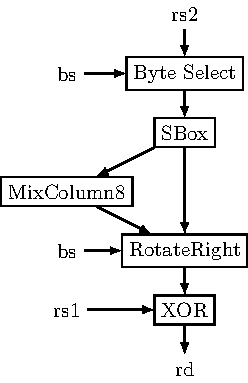
\includegraphics[width=0.45\linewidth]{img/aes32.pdf}}
        \subcaptionbox{SM4}
        {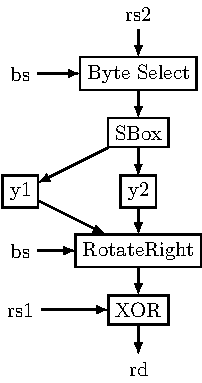
\includegraphics[width=0.35\linewidth]{img/sm4.pdf}}
      \end{figure}
    \end{column}
  \end{columns}
\end{frame}

\begin{frame}{架构总览:五级流水线}
  \begin{center}
    \begin{tikzpicture}[x=2cm]
      \node[draw,thick,fill=white] (IF) at (-2,0) {IF};
      \node[draw,thick,fill=white] (ID) at (-1,0) {ID};
      \node[draw,thick,fill=white] (EXE) at (0,0) {EXE};
      \node[draw,thick,fill=white] (MEM) at (1,0) {MEM};
      \node[draw,thick,fill=white] (WB) at (2,0) {WB};
      \node[draw,thick,fill=white,text=blue] (ALU) at (0,0) {ABLU};
      \node[draw,thick,fill=white,text=red] (Crypto) at (0,1) {NIST/商密};
      \draw[->,thick] (IF) -- (ID);
      \draw[->,thick] (MEM) -- (WB);
      \draw[->,thick] (ID) -- (ALU);
      \draw[->,thick] (ALU) -- (MEM);
      \draw[->,thick] (ID) -- (Crypto);
      \draw[->,thick] (Crypto) -- (MEM);
    \end{tikzpicture}
  \end{center}
  \begin{itemize}
    \item 经典五级流水线: 取指,译码,执行,访存,写回
    \item 我的工作:在执行阶段\begin{itemize}
    \item 增加了NIST/商密密码单元
    \item 将 ALU 替换为 ABLU (算术位运算逻辑单元)
    \end{itemize}
    \item 具体实现参考毕业论文
  \end{itemize}
\end{frame}

\begin{frame}{加速结果}
  \begin{itemize}
    \item 为了测试加速效果,给 OpenSSL 贡献了 AES, SM4, SM3 加速实现\footnote{\texttt{\#18197, \#18267, \#18275, \#18285, \#18287, \#18289, \#18290, \#18308, \#18309}}
    \item 2 到 4 倍的加速比
    \item 密码单元的面积代价与一个乘法器相似
  \end{itemize}
  \begin{figure}
    \centering
    \subcaptionbox{AES-256-CTR}
    {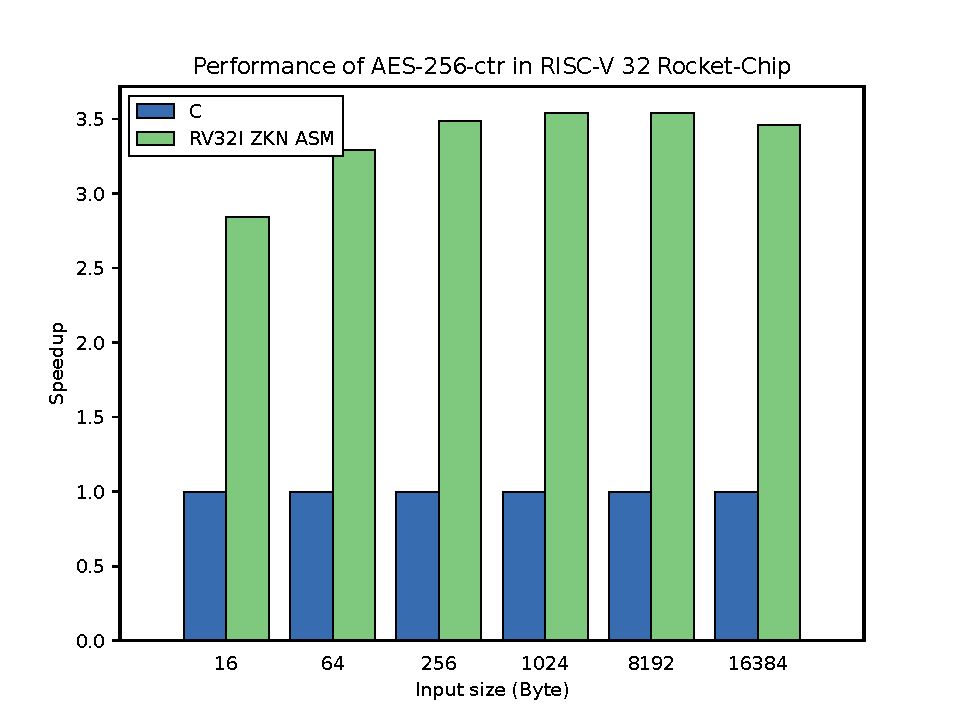
\includegraphics[width=0.3\linewidth]{img/aes-256-ctr.pdf}}
    \subcaptionbox{SM4-CTR}
    {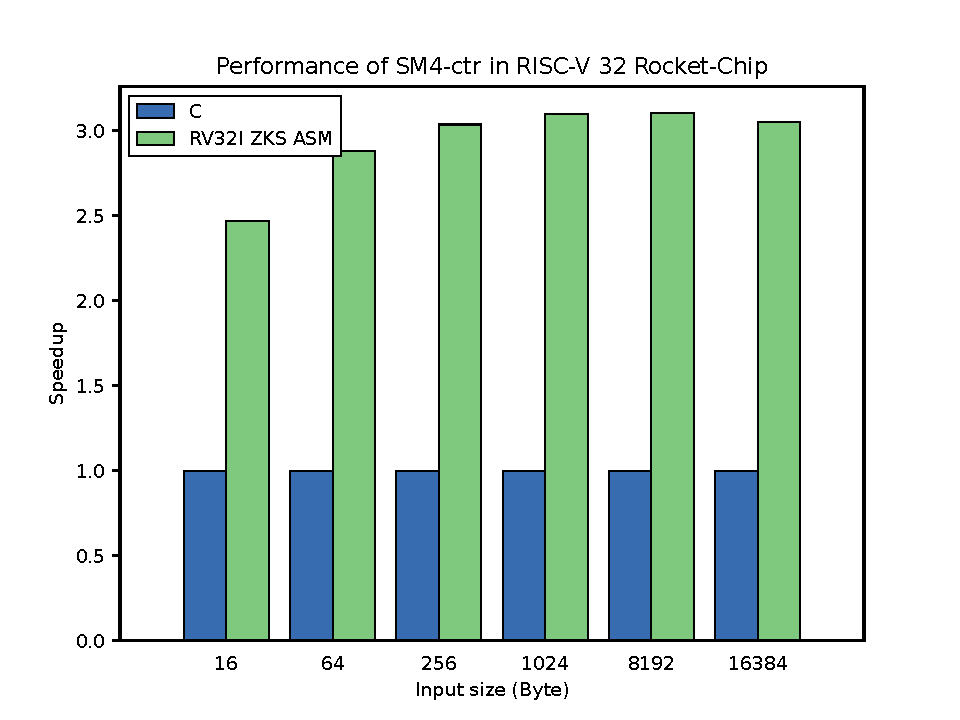
\includegraphics[width=0.3\linewidth]{img/sm4-ctr.pdf}}
    \subcaptionbox{SHA512}
    {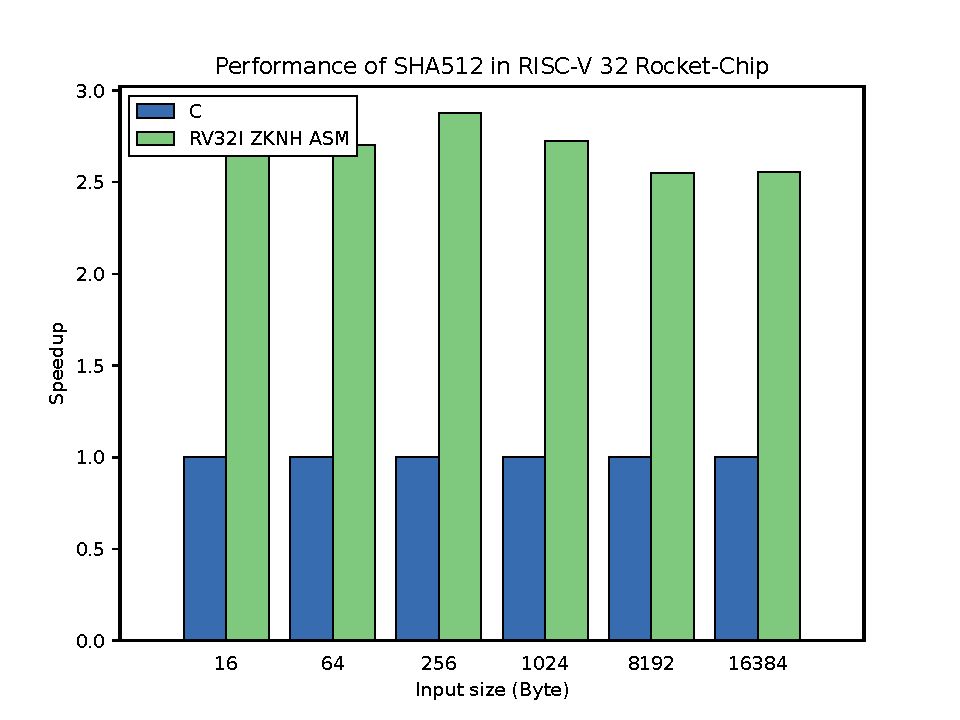
\includegraphics[width=0.3\linewidth]{img/sha512-rv32.pdf}}
  \end{figure}
\end{frame}

\subsection{蒙哥马利模乘加速器}

\begin{frame}{公钥密码学的运算}
  \begin{itemize}
    \item<1-> 以 RSA4096 为例
    \item<1-> 密钥生成\begin{itemize}
      \item 选取两个 2048 位的素数 $p$ 与 $q$
      \item 计算 4096 位整数 $n=pq$
      \item 计算 $\Phi(n)=(p-1)(q-1)$
      \item 选择 $e = 65537$(经典值)
      \item 计算 $d = e^{-1} \pmod{\Phi(n)}$
    \end{itemize}
    \item<1-> 私钥 $(d, n)$,公钥 $(e, n)$
    \item<2-> 签名\begin{itemize}
      \item 消息 $m$
      \item 私钥签名 $c = m ^ {d} \pmod{n}$
      \item 验证签名 $c ^ {e} \equiv m^{de} \equiv m \pmod {n}$
    \end{itemize}
    \item<3-> 核心运算为 4096 位模幂,由一系列「模乘」组成
  \end{itemize}
\end{frame}

\begin{frame}{蒙哥马利模乘算法}
  \begin{itemize}
    \item<1-> 输入 4096 位 $a, b, N$,运算 $ab \pmod{N}$,其中 N 为奇数
    \item<1-> 难点:怎么对 $N$ 取模
    \item<2-> 思路:与其对 $N$ 取模,不如对一个「好」数字取模
    \item<3-> 注意到,在模数为 $2^w$ 时,取模为截取最后 $w$ 位,除法为向右位移 $w$ 位
    \item<3-> 选取 $R = 2^{4096}$
    \item<4-> 预先运算好 $\mu = -N^{-1} \pmod{R}$
    \item<4-> 我们先计算 $q = \mu(ab \pmod{R}) \pmod {R}$
    \item<4-> 再计算 $C = (P+Nq) / R$
    \item<4-> 注意到以上过程中运算主要为 4096 位乘法,取模与除法没有消耗
    \item<4-> 可得 $C = abR^{-1} \pmod{N}$,离 $ab \pmod{N}$ 只有一步之遥
  \end{itemize}
\end{frame}

\begin{frame}{蒙哥马利模乘加速器}
  \begin{itemize}
    \item 又观察到,乘法由加法组成(教科书算法)
    \item 即 $ab = a_0b + a_1b\cdot 2^1 + a_2b\cdot 2^2 + \cdots$
    \item 加速器中只需要做 4096 位加法
  \end{itemize}
  \begin{figure}
    \centering
    \begin{tikzpicture}[x=1cm]
      \node[draw,thick,minimum width=8cm] (adder) at (0,0) {4096 位加法器};
      \node[draw,thick,minimum width=1.8cm] (T) at (-3,1) {$T$}; 
      \node[draw,thick,minimum width=1.8cm] (b) at (-1,1) {$b$}; 
      \node[draw,thick,minimum width=1.8cm] (N) at (1,1) {$N$}; 
      \node[draw,thick,minimum width=1.8cm] (bN) at (3,1) {$b+N$};
      \node[draw,thick,minimum width=1.8cm] (Tp) at (0,-1) {$T'$}; 
      \draw[->,thick] (adder) -- (Tp) -- (-5,-1) -- node[left] {更新} (-5,1) -- (T);
      \draw[->,thick] (T) -- (adder);
      \draw[->,thick,dashed] (b) -- (adder);
      \draw[->,thick,dashed] (N) -- (adder);
      \draw[->,thick,dashed] (bN) -- (adder);
      %
      \node[draw,thick,minimum width=1.8cm] (A) at (6,0.5) {$a$};
      \node[draw,thick,minimum width=1.8cm] (ctrl) at (6,-0.5) {控制逻辑};
      \draw[->,thick] (A) -- (ctrl);
      \draw[->,thick] (ctrl) -- (adder.east);
    \end{tikzpicture}
    \caption{加速器架构}
  \end{figure}
\end{frame}

\begin{frame}{使用 2048 位加速器运算 RSA4096}
  \begin{itemize}
    \item<1-> 4096 位加法器太贵了,能不能便宜点
    \item<1-> 注意到 RSA4096 中,$p$ 与 $q$ 只有 2048 位的
    \item<2-> 中国剩余定理\begin{itemize}
      \item 将 $m^d \pmod N$ 通过以下方式运算
      \item 预先计算 $d_p = d\pmod{p}$, $d_q = d\pmod{q}$, $q_{inv} = q^{-1} \pmod p$ 作为私钥的一部分
      \item 计算 $S_p = m^{d_p}\pmod{p}$
      \item 计算 $S_q = m^{d_q}\pmod{q}$
      \item 计算 $h = q_{inv}\cdot(S_p - S_q) \pmod{p}$
      \item 计算 $S = S_q + h\cdot q \pmod{N}$
    \end{itemize}
    \item<2-> 可以注意到前三步运算为 2048 位模乘
    \item<3-> 最后的 4096 位模乘基于其特殊性质,也可以使用 2048 位模乘实现\only<3->\footnote{参考党凡等人的 xRSA:\url{https://dang.fan/publication/icpads21-xrsa/}}
  \end{itemize}
\end{frame}

\begin{frame}{可配置的加速器}
  \begin{itemize}
    \item 该加速器由叶泽文用 Chisel 编写,高度可配置
    \item 可以较为方便地生成诸如 4096,2048,1024,256 位加速器,面积与应用各有不同
    \item 资源充足时,可以生成 2048 位加速器以支持 RSA4096
    \item 资源较少时,可以生成 1024 位加速器以支持 RSA2048
    \item 资源匮乏时,可以生成 256 位加速器支持椭圆曲线密码学,例如 Ed25519,NIST P-256
    \item 较大的加速器也支持较小的算法,例如 2048 位加速器也支持 Ed25519
  \end{itemize}
\end{frame}

\subsection{USB 1.1 外设} % 突出一个能用就行 % 给个图
\begin{frame}{为什么要做 USB 外设}
  \begin{itemize}
    \item rocket-chip-blocks 中没有相应实现
    \item 其余实现,并不能满足需求\begin{itemize}
      \item 要么只有物理部分
      \item 要么只有控制器
      \item 要么难以接上总线
      \item 要么需要自己写驱动以适配协议栈
    \end{itemize}
    \item 我个人对 USB 较为感兴趣,想做个外设练练手
    \item 结论:自己写
  \end{itemize}
\end{frame}

\begin{frame}{USB 1.1 够用吗}
  \begin{itemize}
    \item 常见误区:签名 1G 的文件,需要将文件全部传输到硬件密钥上
    \item 只需要传输文件的哈希以其他元数据,往往在几百字节
    \item USB 1.1 的 12Mbps 传输速率完全够用
  \end{itemize}
\end{frame}

\begin{frame}{USB 外设架构}
  \begin{center}
    \begin{tikzpicture}[x=2.5cm]
      \node[draw,thick,minimum height=1.5cm] (transaction) at (0,0) {Transaction};
      \node[draw,thick] (packetRx) at (1,0.5) {PacketRx};
      \node[draw,thick] (packetTx) at (1,-0.5) {PacketTx};
      \node[draw,thick,minimum height=1.5cm] (IOBUF) at (1.8,0) {IOBUF};
      \node (DP) at (2.5,0.5) {D$+$};
      \node (DN) at (2.5,-0.5) {D$-$};
      \node[draw,thick] (rxfifo) at (-1,2) {\ RX FIFO\ \ };
      \node[draw,thick] (txfifo0) at (-1,1) {TX FIFO 0};
      \node[draw,thick] (txfifo1) at (-1,0) {TX FIFO 1};
      \node[draw,thick] (txfifo2) at (-1,-1) {TX FIFO 2};
      \node[thick] (txfifo3) at (-1,-2) {...};
      \node (regmap) at (-1.5,2.7) {regmap};
      \draw[thick,dashed] (regmap) -- (-1.5,-2.2);
      %
      \draw[thick,->] (transaction.east |- 52, -0.5) -- (packetTx);
      \draw[thick,->] (packetRx) -- (transaction.east |- 52, 0.5);
      \draw[thick,->] (IOBUF.west |- 52, 0.5) -- (packetRx);
      \draw[thick,->] (packetTx) -- (IOBUF.west |- 52, -0.5);
      \draw[thick,<->] (IOBUF.east |- 52, 0.5) -- (DP);
      \draw[thick,<->] (IOBUF.east |- 52, -0.5) -- (DN);
      %
      \node[thick,draw] (core) at (-2.5,0) {核心};
      \draw[double,<->] (-1.6,0) -- node[above] {tilelink} (-2.2,0);
    \end{tikzpicture}
  \end{center}
\end{frame}

\begin{frame}{最终结果}
  \begin{itemize}
    \item 用 Chisel 编写,自由配置 EP 数量
    \item Linux 能识别
  \end{itemize}
  \begin{figure}
    \centering
    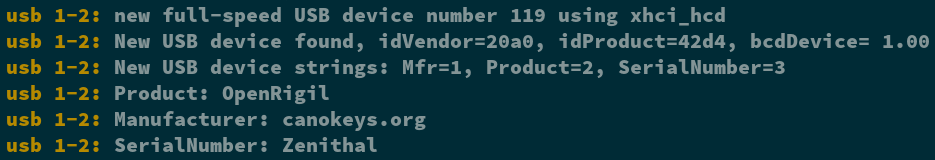
\includegraphics[width=0.8\textwidth]{img/usb.png}
    \caption{Linux 识别 USB 设备}
  \end{figure}
\end{frame}

\subsection{完整系统搭建} % all in chisel (how about all in rust)
\begin{frame}{完整系统}
  \begin{columns}
    \begin{column}{0.5\textwidth}
      \only<1>{硬件部分}
      \only<2>{软件部分}
      \begin{itemize}
        \only<1>{\item 片上系统\begin{itemize}
          \item 单核 RV32IMACZk rocket
          \item 64KB D\$ 作为内存
          \item 2048 位蒙哥马利模乘加速器
          \item USB, SPI, UART(供调试)
          \item 288KB ROM 用于放置固件
        \end{itemize}
        \item 片外 SPI NOR Flash,放置私钥
        \item USB 通过 GPIO 引出}
        \only<2>{\item 密码学库\begin{itemize}
          \item 硬件加速 Ed25519/RSA2048/RSA4096
          \item 其余密码学操作暂借自 MbedTLS
          \item 之后会从 OpenSSL 移植自己写的 AES
        \end{itemize}
        \item 协议栈:canokey-core\begin{itemize}
          \item 支持 FIDO2/OATH/OpenPGP/PIV
          \item 移植了 USB/SPI/UART 驱动
        \end{itemize}}
      \end{itemize}
    \end{column}
    \begin{column}{0.5\textwidth}
      \begin{center}
        \begin{tikzpicture}
          \draw[thick] (-0.1, 0.1) -- (-0.1, 3.0) -- (-3.0, 3.0) -- (-3.0, 0.1) -- (-0.1, 0.1);
          \draw[thick] (0.1, 0.1) -- (0.1, 3.0) -- (3.0, 3.0) -- (3.0, 0.1) -- (0.1, 0.1);
          \draw[thick] (-0.1, -0.1) -- (-0.1, -3.0) -- (-3.0, -3.0) -- (-3.0, -0.1) -- (-0.1, -0.1);
          \draw[thick] (0.1, -0.1) -- (0.1, -3.0) -- (3.0, -3.0) -- (3.0, -0.1) -- (0.1, -0.1);
          \node (core) at (-1.5, 2.5) {核/加速器};
          \node (pheri) at (1.5, 2.5) {外设};
          \node (Crypto) at (-1.5, -0.5) {密码学库};
          \node (Proto) at (1.5, -0.5) {协议栈};
          %
          \node[align=center] (rocket) at (-1.5, 2) {\color{brown}rocket-chip};
          \node[align=center] (blocks) at (1.5, 2) {\color{brown}blocks};
          \node[align=center] (canokey) at (1.5, -1) {\color{brown}canokey-core};
          %
          \node[align=center] (zk) at (-1.5, 1) {{\color{black!40!green}RV32IMAC}{\color{cyan}Zk} \\ {\color{cyan}MMM 加速器}};
          \node[align=center] (peri) at (1.5, 1) {{\color{cyan}USB} \\ {\color{black!40!green}SPI} \\ {\color{black!40!green}UART}};
          \node[align=center] (crypto) at (-1.5, -2) {\color{cyan}RSA ECC \\ \color{cyan}AES \color{black!40!green}SHA};
          \node[align=center] (proto) at (1.5, -2) {\color{black!40!green}FIDO2 OATH \\ \color{black!40!green}OpenPGP PIV};
        \end{tikzpicture}
      \end{center}
    \end{column}
  \end{columns}
\end{frame}

\section{FPGA 原型与实验}
\begin{frame}{FPGA 原型}
  \begin{columns}
    \begin{column}{0.5\textwidth}
      \begin{itemize}
        \item 开发板:Arty A7-100T
        \item 主要特点:拥有大量 GPIO
        \item 关于 USB 的物理条件\begin{itemize}
          \item 需要一个 1.5K 上拉电阻
          \item 板子上部分 IO 拥有上拉电阻
          \item 可以直接使用杜邦线
        \end{itemize}
        \item 一块 USB 转接板,用于杜邦线到 USB 公头的转换
        \item 板上有 16MB 的 SPI NOR Flash,用于放置 bitstream 以及供软件使用
      \end{itemize}
    \end{column}
    \begin{column}{0.5\textwidth}
      \begin{figure}
        \centering
        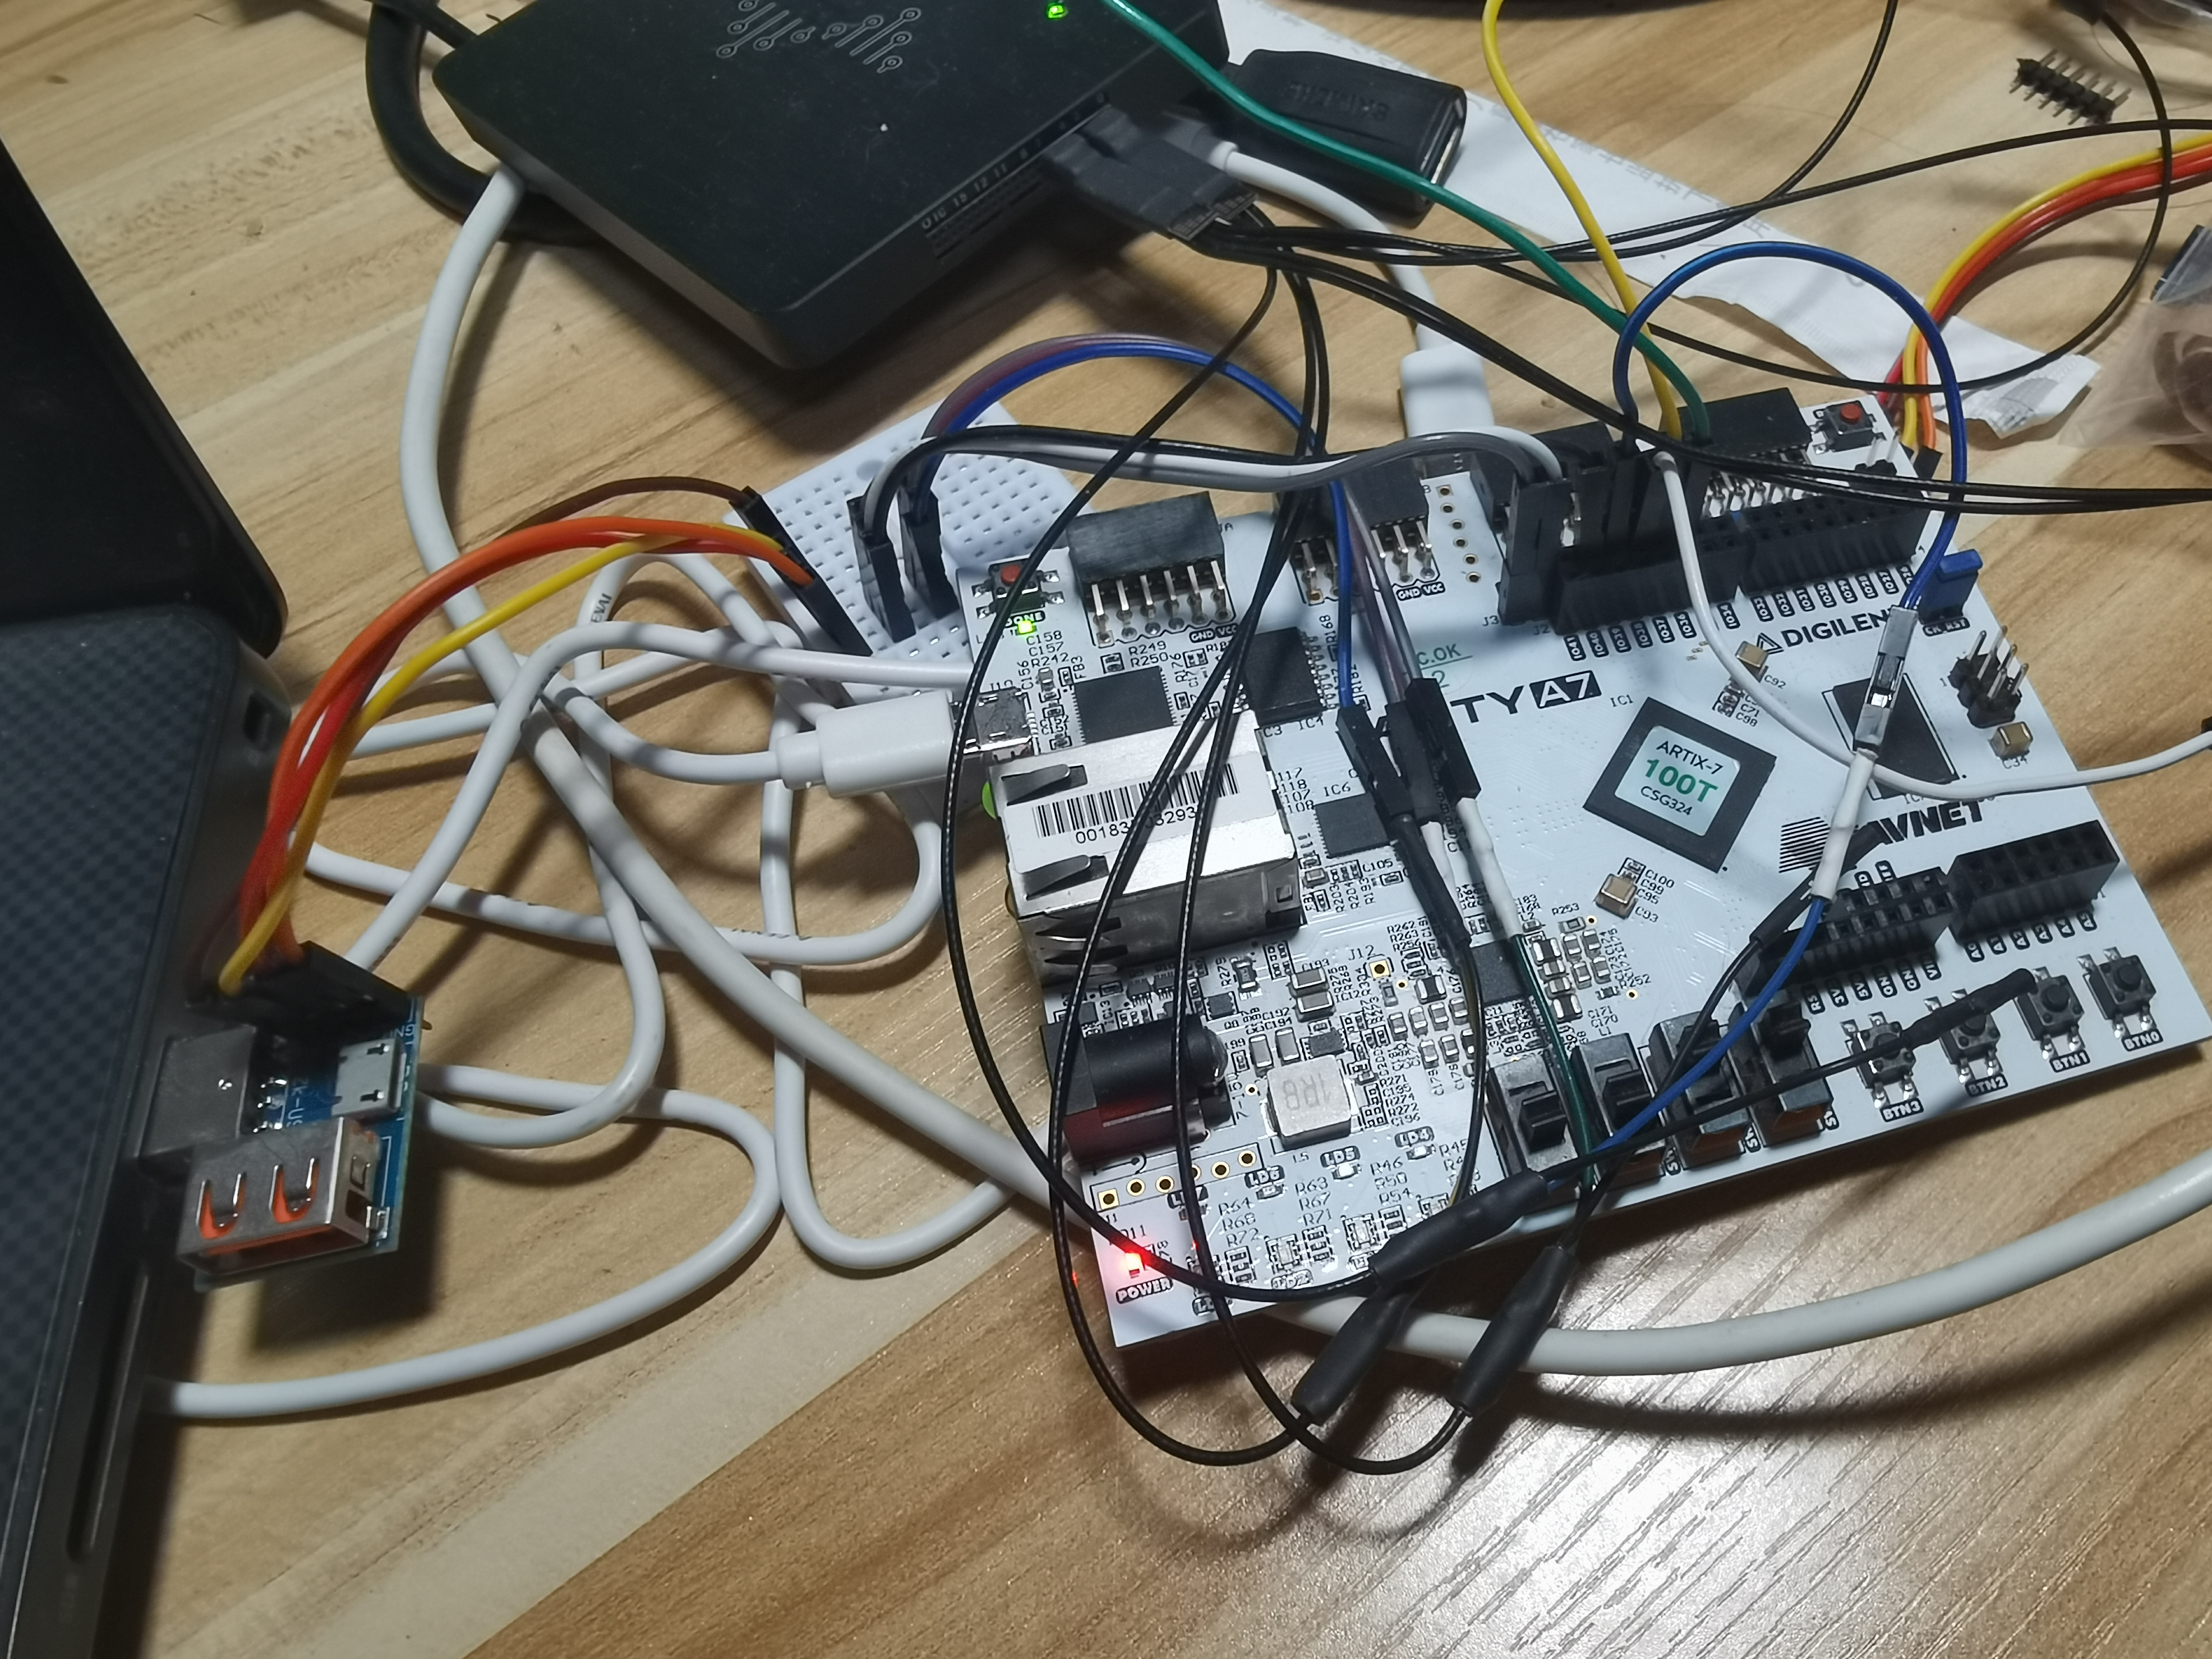
\includegraphics[width=\textwidth]{img/fpga.jpg}
        \caption{实验现场}
      \end{figure}
    \end{column}
  \end{columns}
\end{frame}

\begin{frame}{运行参数}
  \begin{columns}
    \begin{column}{0.5\textwidth}
      \begin{itemize}
        \item 60MHz\begin{itemize}
          \item USB 1.1 12Mbps 的倍数
        \end{itemize}
        \item 53\% LUT(33886/63400) \begin{itemize}
          \item 核、总线、外设 15\%
          \item 2048 位加速器 38\%
          \item 如果选择 256 位加速器,5\%
        \end{itemize}
        \item 84\% BRAM\begin{itemize}
          \item 64K RAM 13\%
          \item 288K ROM 71\%
        \end{itemize}
      \end{itemize}
    \end{column}
    \begin{column}{0.5\textwidth}
      \begin{figure}
        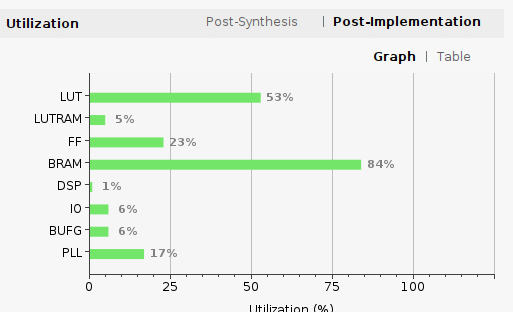
\includegraphics[width=0.9\textwidth]{img/utilization.png}
      \end{figure}
    \end{column}
  \end{columns}
\end{frame}

\begin{frame}{试验结果}
  \begin{table}
    \centering
    \caption{各个算法时间结果}
    \begin{threeparttable}
    \begin{tabular}{crrr}
      \toprule
      算法 & 软件运算 & 硬件加速(签名时间) & GPG 签名整体延迟\\
      \midrule
      Ed25519 & 2.5s & 0.1s & 0.45s\\
      RSA2048 & 4.4s & 0.5s & 1.07s\\
      RSA4096 & 23s & 2.63s & 3.00s\\
      \bottomrule
    \end{tabular}
    \end{threeparttable}
    \label{tab:sbox-area}
  \end{table}
\end{frame}

\section{缺陷与讨论}
\begin{frame}{缺陷与声明(Disclaimer)}
  \begin{itemize}
    \item 并不安全\begin{itemize}
      \item 没有做到密码学硬件「安全」密钥
      \item 事实上,要做到安全还需要更多工作,例如\begin{itemize}
        \item 片外 Flash 的保护
        \item 安全启动
        \item 密码学运算的侧信道问题
        \item 代码是否内存安全,协议栈是否有漏洞
      \end{itemize}
      \item 是一个展示,一个讨论的基础
      \item 建议:不用在生产环境上,供研究与参考
    \end{itemize}
    \item 缺少功能\begin{itemize}
      \item 密码学安全的随机数发生器(CSPRNG) % FIDO 需要这个
      \item 我不保证能做到所以没做,这是个单独的话题
      \item 要真正使用,还需要接入相应的 IP
    \end{itemize}
  \end{itemize}
\end{frame}

\begin{frame}{讨论}
  \begin{itemize}
    \item 隔壁项目:谷歌的 OpenTitan\begin{itemize}
      \item 也是 RISC-V,也是开源硬件,也有密码学加速器
      \item 我们并不是独一家
      \item 完全能做到和我们一样的事情,为什么我们做了呢
      \item 因为我们能做
    \end{itemize}
    \item 这个项目未来会如何\begin{itemize}
      \item 没有答案
      \item 业余慢慢做
      \item 在社区的反馈与支持前进
    \end{itemize}
  \end{itemize}
\end{frame}

\end{document}

% vim: nospell
